\documentclass[12pt]{report}
\usepackage{mathtools, amsthm, mathpazo, epic, eepic, color, paralist, array}
\usepackage[margin=1in]{geometry}
\usepackage{tikz}
\pagestyle{empty}

\begin{document}


\section*{Inverse Functions and L'H\^opital's Rule}

\paragraph{Section 7.1}

\begin{itemize}
\item Remove the last sentence of the first paragraph: \emph{Functions that are not...} 

\item Remove all of the second paragraph except the ast sentence, which should be appended to the end of the first paragraph.

\item Add the following boxed material after the new first paragraph:

For a one-to--one function $f$, 
\begin{enumerate}
\item The domain of $f^{-1}$ is the range of $f$; the range of $f^{-1}$ is the domain of $f$.
\item $f^{-1}(f(x))=x$ for all $x$ in the domain of $f$.
\item $f(f^{-1}(x))=x$ for all $x$ in the domain of $f^{-1}$.
\item The graph of $y=f^{-1}(x)$ is the reflection across $y=x$ of the graph of $y=f(x)$. 
\item $y=f^{-1}(x)$ if and only if $f(y)=x$ and $y$ is in the domain of $f$.
\end{enumerate}

\item The video link should come after this box, but before the next paragraph, which introduces the first example.

\item Move figure 2.29 from the original APEX to here.

\item I'm going to be radical and suggest removing everything from \emph{To find the inverse...} in the middle of page 342 through the end of Example 2. This is entirely algebra. Even worse, it's algebra that students won't ever use in the calculus sequence. Objectors should feel free to write their own material.

\item Replace the paragraph about $f(x)=x^2$ in the middle of page 343 with the following:

\begin{quote}
\subsection*{Functions that are not one-to-one.}

Unfortunately, not every function we would like to find an inverse for is one-to-one. For example, the function $f(x)=x^2$ is not one-to-one because $f(-2)=f(2)=4$. If $f^{-1}$ is an inverse for $f$, then $f^{-1}(f(-2))=-2$ implies that $f^{-1}(4)=-2$. On the other hand, $f^{-1}(f(2))=2$, so $f^{-1}(4)=2$. We cannot have it both ways if $f^{-1}$ is a function, so no such inverse exists. We can find a partial solution to this dilemma by restricting the domain of $f$. There are many possible choices, but traditionally we restrict the domain to the interval $[0,\infty)$. The function $f^{-1}(x)=\sqrt x$ is now an inverse for this restricted version of $f$. 
\end{quote}

\item Change $\arcsin$ to $\sin^{-1}$ everywhere, $\arctan$ to $\tan^{-1}$, etc. Add marginal comment about the alternate notation.

\item Move the graph of the sine function into the margin (and number?)

\item Combine the graphs of $y=\sin x$ and $y=\sin^{-1}x$ and add the line $y=x$. They should also be in the margin.

\item Make similar changes to the discussion of $\tan^{-1}$.

\item After the discussion of $\tan^{-1}$, add the following:

\begin{quote}
The other inverse trigonometric functions are defined in a similar fashion. The resulting domains and ranges are summarized in the following:
\end{quote}

\item Move figure 7.4 from page 349 here. Add \emph{restricted} to label on domain of trig functions in header.

\item Add the following

\begin{quote}
{\bfseries Example 2.} Find exact values for the following.
\begin{enumerate}
\item $\tan^{-1}(1)$
\item $\cos(\sin^{-1}(\sqrt 3/2))$
\item $\sin^{-1}(\sin(7\pi/6))$
\item $\tan(\cos^{-1}(11/15))$
\end{enumerate}
\par
{\bfseries Solution.}
\begin{enumerate}
\item $\tan^{-1}(1)=\pi/4$
\item $\cos(\sin^{-1}(\sqrt3/2))=\cos(\pi/3)=1/2$
\item Since $-7\pi/6$ is not in the range of the inverse sine function, you should be careful with this one. \[\sin^{-1}(\sin(7\pi/6))=\sin^{-1}(-1/2)=-\pi/6\]
\item Since we don't know the value of $\cos^{-1}(11/15)$, we let $\theta$ stand for this value. We know that $\theta$ is an angle between $0$ and $\pi$ and that $\cos(\theta)=11/15$. We use this information to construct a right triangle with angle $\theta$, where the adjacent side over the hypotenuse must equal $11/15$:

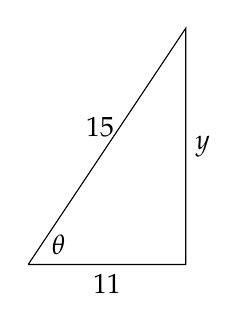
\begin{tikzpicture}
\draw (0,0) node[above right]{\ \ $\theta$} -- (1,0) node[below]{11} -- (2,0) -- (2,1.5) node[right]{$y$} -- (2,3) -- (1,1.5) node[above]{15 \ \ } -- (0,0);
\end{tikzpicture}
\end{enumerate}

Applying the Pythagorean Theorem we find that \[y=\sqrt{15^2-11^2}=\sqrt{104}=2\sqrt{26}.\]
Finally, we have: \[\tan(\cos^{-1}(11/15))=\tan(\theta)=\frac{2\sqrt{26}}{11}\]
\end{quote}

\item Remove problems 9-11.

\item Add the following problems.

\begin{itemize}
\item[] In exercises 9-12, find a restriction of the domain of the given function on which the function will have an inverse.
\begin{itemize}
\item[9.] $f(x)=\sqrt{16-x^2}$
\item[10.] $g(x)=\sqrt{x^2-16}$
\item[11.] $r(t)=t^2-6t+9$
\item[12.] $f(x)=\frac{1-\sqrt x}{1+\sqrt x}$
\end{itemize}
\item[] In exercises 13-19 find the exact value.
\begin{itemize}
\item[13.] $\tan^{-1}(0)$
\item[14.] $\tan^{-1}(\tan(\pi/7))$
\item[15.] $\cos(\cos^{-1}(-1/5))$
\item[16.] $\sin^{-1}(\sin(8\pi/3))$
\item[17.] $\sin(\tan^{-1}(1))$
\item[18.] $\cos(\tan^{-1}(3/7))$
\item[19.] $\sec(\sin^{-1}(-3/5))$
\end{itemize}
\end{itemize}

\end{itemize}

\paragraph{Section 7.2}

\begin{itemize}
\item In the first line of the paragraph beginning \emph{In Figure 7.3 we see...}, $f^{-1}=\sin^{-1} x$ should be $f^{-1}(x)=\sin^{-1}x$
\item Remove figure 7.4 on page 349.
\item Remove Example 2 as well as the paragraph introducing it. This is done in the next section and fits better there.
\item Add the following material to the end of the section.

{\color{blue}
\paragraph{Example 2.} Find the derivatives of the following functions.

\begin{enumerate}
\item $f(x)=\cos^{-1}(x^2)$
\item $\displaystyle g(x)=\frac{\sin^{-1}x}{\sqrt{1-x^2}}$
\item $f(x)=\sin^{-1}(\cos x)$
\end{enumerate}

\paragraph{Solutions.}

\begin{enumerate}
\item We use Theorem 47 and the Chain Rule to find: \[f'(x)=-\frac{1}{\sqrt{1-x^2}}(2x)=- \frac{2x}{\sqrt{1-x^2}}\]
\item We use Theorem 47 and the Quotient Rule to compute: 
\begin{equation*}
\begin{split}
g'(x)&=\frac{\left(\frac 1{\sqrt{1-x^2}}\right)\sqrt{1-x^2} - (\sin^{-1} x)\left( \frac 1{2\sqrt{1-x^2}} (-2x)\right)}{\sqrt{1-x^2}^2}\\
&=\frac{\sqrt{1-x^2}+x\sin^{-1}x}{\sqrt{1-x^2}^3}\\
\end{split}
\end{equation*}
\item We apply Theorem 47 and the Chain Rule again to compute:
\begin{equation*}
\begin{split}
f'(x)&=\frac{1}{\sqrt{1-\cos^2x}}(-\sin x)\\
&=\frac{-\sin x}{\sqrt{\sin^2x}}\\
&=\frac{-\sin x}{\sin x}\\
&=-1\\
\end{split}
\end{equation*}
\end{enumerate}

Theorem 47  allows us to integrate some functions that we could not integrate before. For example, \[\int\frac{dx}{\sqrt{1-x^2}}=\sin^{-1}x+C.\] Combining these formulas with $u$-substitution yields the following:

{\color{red} \bfseries Insert Theorem 46 from page 267 of the original APEX text here, where it becomes Theorem 48?}

We will look at the second part of this theorem. The other parts are similar and are left as exercises.

First we note that the integrand involves the number $a^2$, but does not explicitly involve $a$. We make the assumption that $a>0$ in order to simplify what follows. We can rewrite the integral as follows: \[ \int\frac{dx}{\sqrt{a^2-x^2}} =\int\frac{dx}{\sqrt{a^2(1-(x/a)^2)}}=\int\frac{dx}{a\sqrt{1-(x/a)^2}}\] We next use the subsitution $u=x/a$ and $du=dx/a$ to find compute: 
\begin{equation*}
\begin{split}
\int\frac{dx}{a\sqrt{1-(x/a)^2}} &=\int\frac{a}{a\sqrt{1-u^2}}\,du\\
&=\int \frac{du}{\sqrt{1-u^2}}\\
&=\sin^{-1}u+C\\
&=\sin^{-1}(x/a)+C\\
\end{split}
\end{equation*}

We conclude this section with several examples.

\paragraph{Example 3.} Find the following.
\begin{enumerate}
\item $\displaystyle\int\frac{dx}{100+x^2}$
\item $\displaystyle\int\frac{\sin^{-1} x}{\sqrt{1-x^2}}\,dx$
\item $\displaystyle\int\frac{dx}{x^2+2x+5}$
\end{enumerate}

\paragraph{Solutions.}
\begin{enumerate}
\item $\displaystyle \int \frac{dx}{100+x^2}=\int\frac{dx}{10^2+x^2} =\frac1{10}\tan^{-1}(x/10)+C$
\item We use the substitution $u=\sin^{-1}x$ and $du=\frac{dx}{\sqrt{1-x^2}}$ to find:
\[\int \frac{\sin^{-1}x}{\sqrt{1-x^2}} = \int u\,du =\frac 12 u^2+C=\frac 12 \sin^{-1}x+C\]
\item This does not immediately look like one of the forms in Theorem 48, but we can complete the square in the denominator to see that \[\int\frac{dx}{x^2+2x+5} =\int\frac{dx}{(x^2+2x+1)+4}=\int\frac{dx}{4+(x+1)^2}\] We now use the substitution $u=x+1$ and $du=dx$ to find: \[\int\frac{dx}{(4+(x+1)^2} =\int\frac{du}{4+u^2}=\frac12 \tan^{-1}(u/2)+C =\frac 12\tan^{-1}\left(\frac{x+1}2\right)+C\]
\end{enumerate}

}

\end{itemize}

\paragraph{Section 7.3}

\begin{itemize}

\item Move figures 7.5 \& 7.6 to the margin
\item The information currently on the bottom of page 353 should be boxed and read as follows: \par
For $a>0$ the exponential function $f(x)=a^x$ satisfies:
\begin{enumerate}
\item $a^0=1$
\item The domain of $f(x)=a^x$  is $(-\infty,\infty)$ and the range is $(0,\infty)$.
\item $\displaystyle\lim_{x\to\infty} a^x=\begin{cases} \infty & \text{if $a>1$}\\ 0 & \text{if $a<1$}\\ \end{cases}$
\item $\displaystyle\lim_{x\to-\infty} a^x= \begin{cases} 0 & \text{if $a>1$}\\ \infty & \text{if $a<1$}\\ \end{cases}$
\end{enumerate}

\item Remove Example 1, it's really Calc I and we can't do other bases correctly yet. See Example 2 note below.

\item Add the following (boxed) after the first paragraph about general logarithmic functions on page 355:
For $a>0$ and $a\neq 1$ the logarithmic function $f(x)=\log_ax$ satisfies:
\begin{enumerate}
\item The domain of $f(x)=\log_a x$ is $(0,\infty)$ and the range is $(-\infty,\infty)$.
\item $y=\log_ax$ if and only if $a^y=x$.
\item $\displaystyle\lim_{x\to\infty} \log_ax= \begin{cases} \infty & \text{if $a>1$}\\ -\infty & \text{if $a<1$}\\ \end{cases}$
\item $\displaystyle\lim_{x\to0} \log_ax= \begin{cases} -\infty & \text{if $a>1$}\\ \infty & \text{if $a<1$}\\ \end{cases}$
\end{enumerate}

\item Add the line $y=x$ to figure 7.7 and move to margins.

{\color{red} {\bfseries Undue change mentioned in red if you made it.}
\item Under Derivatives of logarithmic functions, replace the first derivation with: \emph{In Section 7.2, Example 2 we found that $\frac{d}{dx}\ln x=\frac1x$.} Remove the word \emph{Now} at the beginning of the next sentence.}

\item Replace part 2 of Example 2 with the following: $f(x)=2^{x^2}$. The solution follows:
We apply the Chain Rule: \[ f'(x)=\left(2^{x^2}\ln 2\right)(2x)=2^{x^2+1}x\ln 2\]

\item Under Antiderivatives, replace the first sentence with: \emph{Combining these new results, we arrive at the following theorem:}

\item Rename Theorem 50 \emph{Derivatives and Antiderivatives of Exponentials and Logarithms}. Then add the following parts: 
\begin{itemize}
\item[$\bullet$] $\frac{d}{dx} e^x=e^x$
\item[$\bullet$] $\frac{d}{dx}a^x=a^x\ln a$
\item[$\bullet$] $\frac{d}{dx} \ln x=\frac 1x$ 
\item[$\bullet$] $\frac{d}{dx}\log_ax=\frac 1{x\ln a}$
\end{itemize}

\item Is Example 5 in Section 8.1 still correct on page 359?
\end{itemize}

\paragraph{Section 7.4}

\begin{itemize}
\item Can the second paragraph be reworked so that the equation $x^2+y^2=1$ fits on a single line? Maybe just spacing?
\end{itemize}

\paragraph{Section 7.5}

\begin{itemize}
\item In part 1(a) of Theoorem 51, it should read \emph{except possibly at $x=a$}

\item Maybe split Theorem 51 back into two theorems?
\end{itemize}

\end{document}
